% ============================================================
%  Rozdział 5 — Manewry
% ============================================================
\section{Manewry}

\begin{tipbox}
\noindent
\begin{minipage}[c]{0.72\linewidth}
  W PrzeWrotce, podobnie jak w kilku innych akademickich klubach kajakowych, praktykuje się tradycję kreślenia palcem znaku wiru na kasku po zanurzeniu ręki w wodzie, jako symboliczne życzenie bezpiecznego spłynięcia.
\end{minipage}
\hfill
\begin{minipage}[c]{0.18\linewidth}
  \centering
  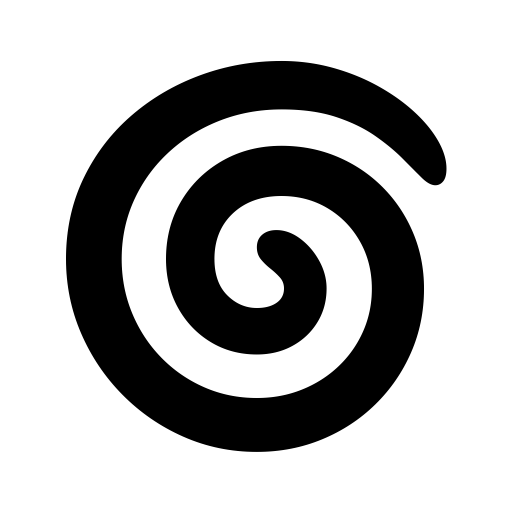
\includegraphics[width=\linewidth]{images/wir.png}
\end{minipage}
\end{tipbox}

% ------------------------------------------------------------
\subsection{Rozgrzewka}
% ------------------------------------------------------------

Dobrze przeprowadzona rozgrzewka w kajakarstwie górskim realnie zmniejsza ryzyko kontuzji
i poprawia kontrolę łódki. Rozgrzewka ma na celu:

\begin{itemize}[leftmargin=1.5em, itemsep=2pt]
  \item podniesienie temperatury ciała,
  \item przygotowanie stawów i mięśni do pracy w wodzie,
  \item aktywację mięśni stabilizujących,
  \item poprawę koordynacji i czucia ciała,
  \item zmniejszenie ryzyka urazów barków, kręgosłupa i nadgarstków,
  \item mobilizację bioder.
\end{itemize}

\begin{tipbox}
  Czas trwania: 10--15 minut, dopasowany indywidualnie.
  Rozgrzewkę wykonujemy \textbf{na lądzie}, przed wejściem do kajaka.
\end{tipbox}


% ------------------------------------------------------------
\subsection{Przechył}
% ------------------------------------------------------------

Przechył kajaka to kontrolowane przechylenie łodzi na bok (na burtę), wykonywane świadomie przez kajakarza za pomocą pracy bioder i odpowiedniego ułożenia ciała. Bezpośrednio wpływa
na stabilność i sterowność — kajak znacznie lepiej reaguje na ruchy wykonywane w lekkim przechyle, a sztywna, napięta postawa utrudnia panowanie nad łodzią.

Przechył polega na \textbf{uniesieniu jednej burty kajaka i dociążeniu drugiej} poprzez pracę bioder i uniesienie jednego kolana, przy jednoczesnym zachowaniu względnie pionowej pozycji tułowia. Ruch powinien wynikać z kontrolowanego „rolowania" bioder, nie z pochylania całego ciała na bok. Głowa powinna pozostawać możliwie blisko osi kajaka — jej wychylenie na stronę przechyłu znacząco zwiększa ryzyko wywrotki.

Wystarczy \textbf{niewielki, kilkustopniowy przechył}, aby kajak zaczął lepiej skręcać i stabilniej zachowywał się na falach. Zbyt duży przechył bez wsparcia wiosłem może
prowadzić do wywrotki.

Wiosło pełni ważną rolę w utrzymaniu równowagi podczas przechyłu — lekkie podparcie o taflę wody pozwala poczuć stabilność kajaka i zmniejsza strach przed przechyleniem.
Z czasem kajakarz uczy się łączyć pracę bioder, tułowia i wiosła w jeden płynny ruch.

% ------------------------------------------------------------
\subsection{Wsiadanie i wysiadanie z kajaka}
% ------------------------------------------------------------

\textbf{Wsiadanie} najlepiej wykonywać na płytkiej wodzie lub z niskiego, stabilnego brzegu. Kajak ustawiamy równolegle do brzegu lub lekko dziobem pod prąd. Wiosło kładzie się
poprzecznie za kokpitem, opierając jedno pióro o brzeg lub dno, a drugie o kajak — tworzy to stabilny punkt podparcia. Następnie:

\begin{enumerate}[leftmargin=1.5em, itemsep=2pt]
  \item Uchwyć jedną ręką krawędź kokpitu, drugą wiosło.
  \item Usiądź najpierw na tylnej części kokpitu.
  \item Wsuwaj nogi do środka kajaka.
  \item Przenoś ciężar ciała płynnie, utrzymując środek ciężkości nisko.
  \item Ustaw stopy na podnóżkach i sprawdź pozycję przed odbiciem od brzegu.
\end{enumerate}

\textbf{Wysiadanie} wykonuje się w zasadzie w odwrotnej kolejności. Po zatrzymaniu kajaka w spokojnym miejscu lub przy brzegu: stabilizuj łódź wiosłem, wysuń nogi z kokpitu, oprzyj je o dno lub brzeg, powoli przenieś ciężar ciała na zewnątrz. Nie wstawaj gwałtownie — najpierw „usiądź na brzegu" kajaka, a dopiero potem wstań.

\begin{tipbox}
  Zarówno przy wsiadaniu, jak i wysiadaniu najważniejsze są spokój i precyzja ruchów. Pośpiech niemal zawsze kończy się wywrotką. Na rzece wybieraj miejsca w cofce lub osłonięte od prądu.
\end{tipbox}

% ------------------------------------------------------------
\subsection{Wiosłowanie}
% ------------------------------------------------------------

\begin{longtable}{>{\bfseries}p{4.2cm} p{4.9cm} p{4.9cm}}
  \toprule
  \textbf{Cecha} & \textbf{Wiosłowanie szerokie} & \textbf{Wiosłowanie pionowe} \\
  \midrule
  \endfirsthead
  \toprule
  \textbf{Cecha} & \textbf{Wiosłowanie szerokie} & \textbf{Wiosłowanie pionowe} \\
  \midrule
  \endhead
  \bottomrule
  \endfoot

  Cel główny
    & Skręcanie kajaka, manewrowanie
    & Przemieszczanie się do przodu, przyspieszanie \\

  Pozycja wiosła
    & Pióro daleko od kajaka, ruch półkolisty
    & Pióro bliżej kajaka, prowadzone wzdłuż kadłuba \\

  Początek ruchu
    & Przy stopach
    & Przy stopach \\

  Koniec ruchu
    & Przy rufie
    & Przy biodrach \\

  Ruch tułowia
    & Obrót całego torsu
    & Stabilizacja torsu, bardziej izolowany ruch ramienia \\

  Pozycja nadgarstka
    & Naturalna, mniej krytyczna
    & Nadgarstek przecina pole widzenia; wymaga kontroli \\
\end{longtable}

% ------------------------------------------------------------
\subsection{Podpórka}
% ------------------------------------------------------------

Technika służąca do utrzymania równowagi i zapobiegania wywrotce w sytuacji, gdy kajak traci stabilność. Polega na krótkim, dynamicznym oparciu pióra wiosła o powierzchnię wody
w celu uzyskania dodatkowego podparcia. Podpórka nie jest ruchem siłowym — opiera się na właściwym ułożeniu ciała, pracy bioder i odpowiednim kącie pióra względem wody.

Wykonuje się ją, gdy kajak zaczyna przechylać się na jedną burtę. Wiosło trzymane jest nisko, przed kajakarzem, a pióro ustawia się \textbf{płasko} na powierzchni wody po stronie
przechyłu. Łokcie pozostają blisko tułowia, nadgarstki w neutralnej pozycji — chroni to stawy przed urazami. Kluczowym elementem jest jednoczesna \textbf{praca bioder}, które
prostują kajak, podczas gdy wiosło daje krótkie, stabilne podparcie.

\begin{tipbox}
  Ruch podpórki jest szybki i krótki — nie chodzi o opieranie się ciężarem ciała na wiośle, lecz o chwilowe „dotknięcie" wody i powrót do normalnego prowadzenia kajaka.
\end{tipbox}

% ------------------------------------------------------------
\subsection{Promowanie i trawers}
% ------------------------------------------------------------

Dwa podstawowe manewry pozwalające bezpiecznie poruszać się w poprzek nurtu rzeki. Oba opierają się na odpowiednim ustawieniu kajaka względem prądu.

\textbf{Promowanie} polega na przepłynięciu kajakiem w poprzek rzeki bez znoszenia przez nurt (lub przy kontrolowanym znoszeniu). Kajak ustawiony jest pod odpowiednim kątem do prądu — dziobem lekko pod nurt — dzięki czemu siła wody napierająca na burtę równoważy
znoszenie w dół rzeki.

Kajakarz utrzymuje stały kąt kajaka i wykonuje regularne, spokojne pociągnięcia wiosłem.

\begin{itemize}[leftmargin=1.5em, itemsep=2pt]
  \item \textbf{Zbyt mały kąt} — brak przemieszczania się w bok lub problem z wyjściem z cofki.
  \item \textbf{Zbyt duży kąt} — nurt „zabiera" dziób, kajak obraca się dziobem w dół rzeki i jest znoszony.
\end{itemize}

W obu manewrach ważna jest zasada: \textbf{Patrz gdzie płyniesz} — przemieszczamy się tam, gdzie skierowana jest nasza głowa i wzrok. Jeśli uporczywie wpatrujemy się w wodę /
nurt, najpewniej się przewrócimy.


% ------------------------------------------------------------
\subsection{Wchodzenie z cofki}`
% ------------------------------------------------------------

\begin{figure}[H]
    \centering
    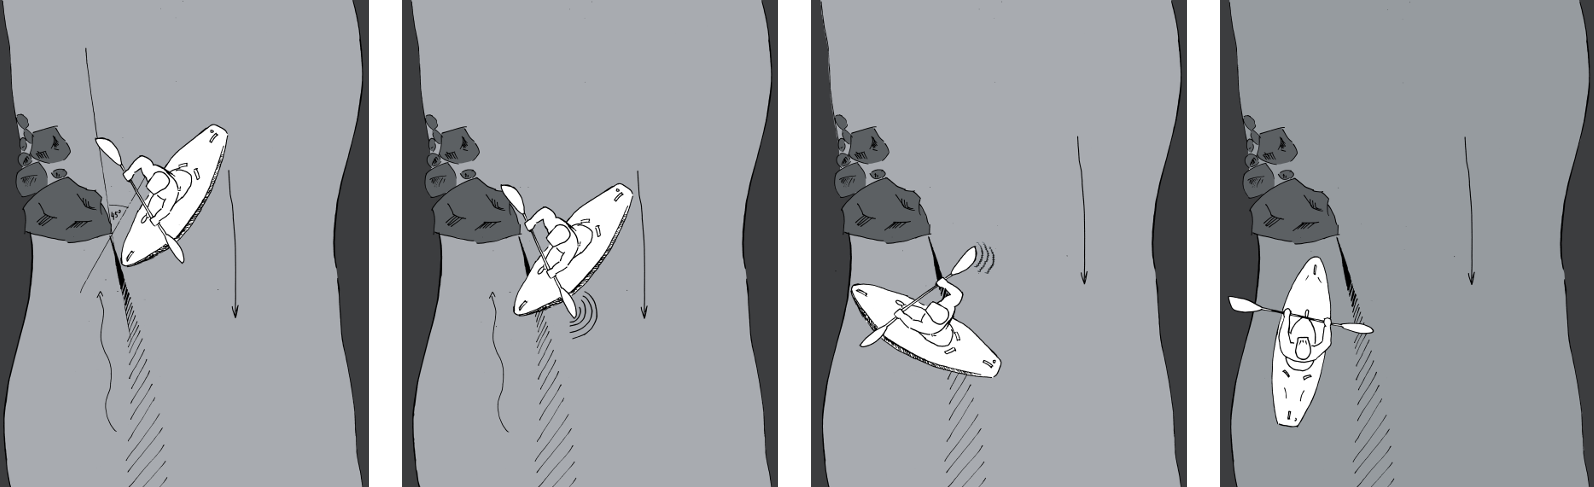
\includegraphics[width=400px]{images/wchodzenie_do_cofki.png}
    \caption{Schemat wejścia do cofki}
\end{figure}

% ------------------------------------------------------------
\subsection{Wychodzenie do cofki}
% ------------------------------------------------------------

\begin{figure}[H]
    \centering
    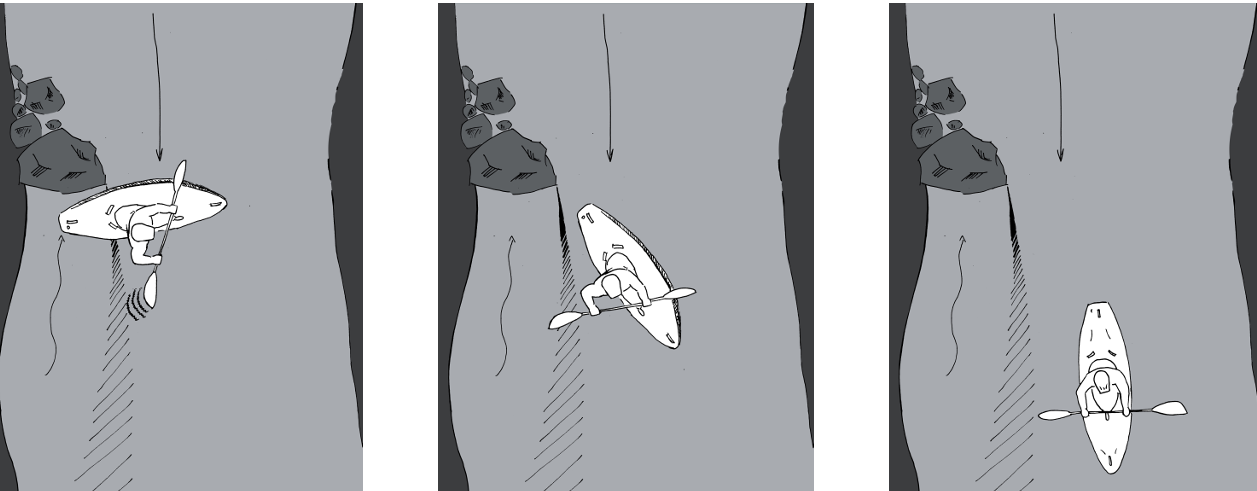
\includegraphics[width=400px]{images/wychodzenie_z_cofki.png}
    \caption{Schemat wyjścia z cofki}
\end{figure}